\documentclass[a4paper,10pt]{scrartcl}
\usepackage[utf8]{inputenc}
\usepackage{graphicx}
\usepackage{listings}
\usepackage{color}
\usepackage[colorlinks=true, pdfborder={0 0 0}, linkcolor=blue, citecolor=magenta]{hyperref}
\usepackage{titlesec}

\titleformat{\section}
  {\Large\bfseries} % format
  {}                % label
  {0pt}             % sep
  {\huge}           % before-code
\setkomafont{sectioning}{\bfseries} % erzeugt Überschriften mit Serifen!!!
\definecolor{mygreen}{rgb}{0,0.6,0}
\definecolor{mygray}{rgb}{0.5,0.5,0.5}
\definecolor{mymauve}{rgb}{0.58,0,0.82}
\lstset{ %
  backgroundcolor=\color{white},   % choose the background color; you must add \usepackage{color} or \usepackage{xcolor}
  basicstyle=\footnotesize,        % the size of the fonts that are used for the code
  breakatwhitespace=false,         % sets if automatic breaks should only happen at whitespace
  breaklines=true,                 % sets automatic line breaking
  captionpos=b,                    % sets the caption-position to bottom
  commentstyle=\color{mygreen},    % comment style
  deletekeywords={...},            % if you want to delete keywords from the given language
  escapeinside={\%*}{*)},          % if you want to add LaTeX within your code
  extendedchars=true,              % lets you use non-ASCII characters; for 8-bits encodings only, does not work with UTF-8
  frame=single,                    % adds a frame around the code
  keepspaces=true,                 % keeps spaces in text, useful for keeping indentation of code (possibly needs columns=flexible)
  keywordstyle=\color{blue},       % keyword style
  language=c++,                 % the language of the code
  morekeywords={*,...},            % if you want to add more keywords to the set
  numbers=left,                    % where to put the line-numbers; possible values are (none, left, right)
  numbersep=5pt,                   % how far the line-numbers are from the code
  numberstyle=\tiny\color{mygray}, % the style that is used for the line-numbers
  rulecolor=\color{black},         % if not set, the frame-color may be changed on line-breaks within not-black text (e.g. comments (green here))
  showspaces=false,                % show spaces everywhere adding particular underscores; it overrides 'showstringspaces'
  showstringspaces=false,          % underline spaces within strings only
  showtabs=false,                  % show tabs within strings adding particular underscores
  stepnumber=2,                    % the step between two line-numbers. If it's 1, each line will be numbered
  stringstyle=\color{mymauve},     % string literal style
  tabsize=2,                       % sets default tabsize to 2 spaces
  title=\lstname                   % show the filename of files included with \lstinputlisting; also try caption instead of title
}
\lstdefinestyle{customc}{
  belowcaptionskip=1\baselineskip,
  breaklines=true,
  frame=L,
  xleftmargin=\parindent,
  language=c++,
  showstringspaces=false,
  basicstyle=\footnotesize\ttfamily,
  keywordstyle=\bfseries\color{green!40!black},
  commentstyle=\itshape\color{purple!40!black},
  identifierstyle=\color{blue},
  stringstyle=\color{orange},
}

%opening
\title{Documentation for the Cancerdynamics Simulator}
\author{Boris Prochnau}

\begin{document}

\maketitle
\tableofcontents
\newpage
%\fontfamily{ppl}\selectfont
\section{General Information}
First I would like to say that I tried to make the code as readable as possible with the knowledge and experience I had at this time. Of curse both grew since than and I would make some things different. Still this documentation is pretty tight coupled to the code and uses the assumption that many variables, function names and some computations should be self-explaining once you know what to look at. \\
Also it seems long ago when I wrote this simulation and I lost my records of notes. That's why I had to reassemble my understanding of the algorithm by explaining the code within the simulation. Some things are still not totally clear.
\begin{figure}
\centering
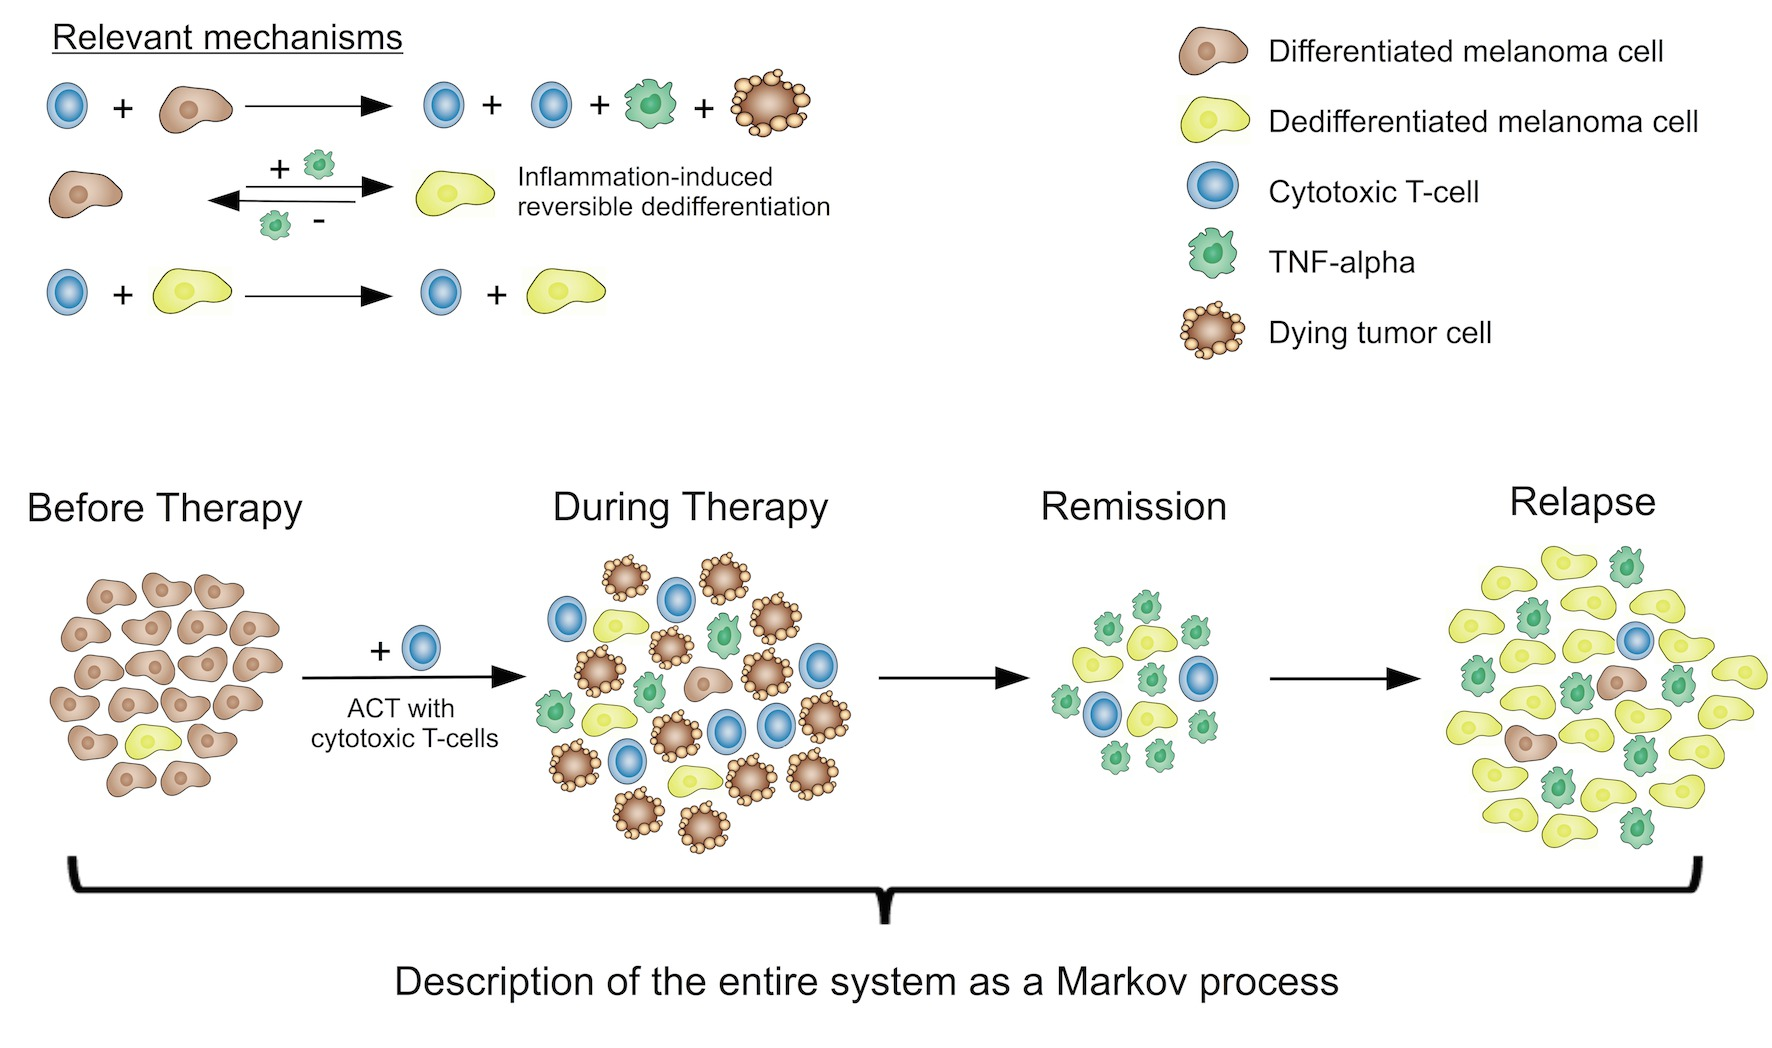
\includegraphics[width=1\linewidth]{Bilder/Schema_Tumor_rescale}
\caption{rescaling Tumor}
\label{fig:Schema_Tumor_rescale}
\end{figure}

\subsection{Work-flow and levels of abstraction}
The simulation works with an algorithm that can be applied repeatedly to changing Data. Every application of the algorithm will modify the data (the given population). So the basically we see the goal of creating a process by displaying the stages of the data after one application of the algorithm. That's why the function containing the algorithm is called 'makeEvolutionStep' (or in older versions just EvolutionStep).\\
The work-flow was separated into different abstraction levels. They can be seen in a depth-diagram (fig. \ref{fig:Tiefendiagram}). 

\subsection{Expressions}
The population consists of members that are grouped by their traits. Each trait represents its own behaviour and doesn't vary between members of this trait. Thats why this algorithm (and the one from my bachelor thesis) works with traits (this means the data structure doesn't know about t-cells or melanoma cells, they are all traits).
The algorithm expects a specific pattern of traits with specific behaviour. It is specified in the 'Musterinstanz.txt' and 'Testinstanz\_kommentiert'. The population is grouped into:
\begin{enumerate}
	\item TNF-$ \alpha $
	\item t-cells
	\item melanoma cells (phenotypes $ \times $ genotypes)		
\end{enumerate}
where every group has their own behaviour within the algorithm, i.e. the t-cells have no possibility to switch like the melanoma cells (see fig. \ref{fig:Schema_Tumor_rescale}).
\begin{figure}
	\centering
	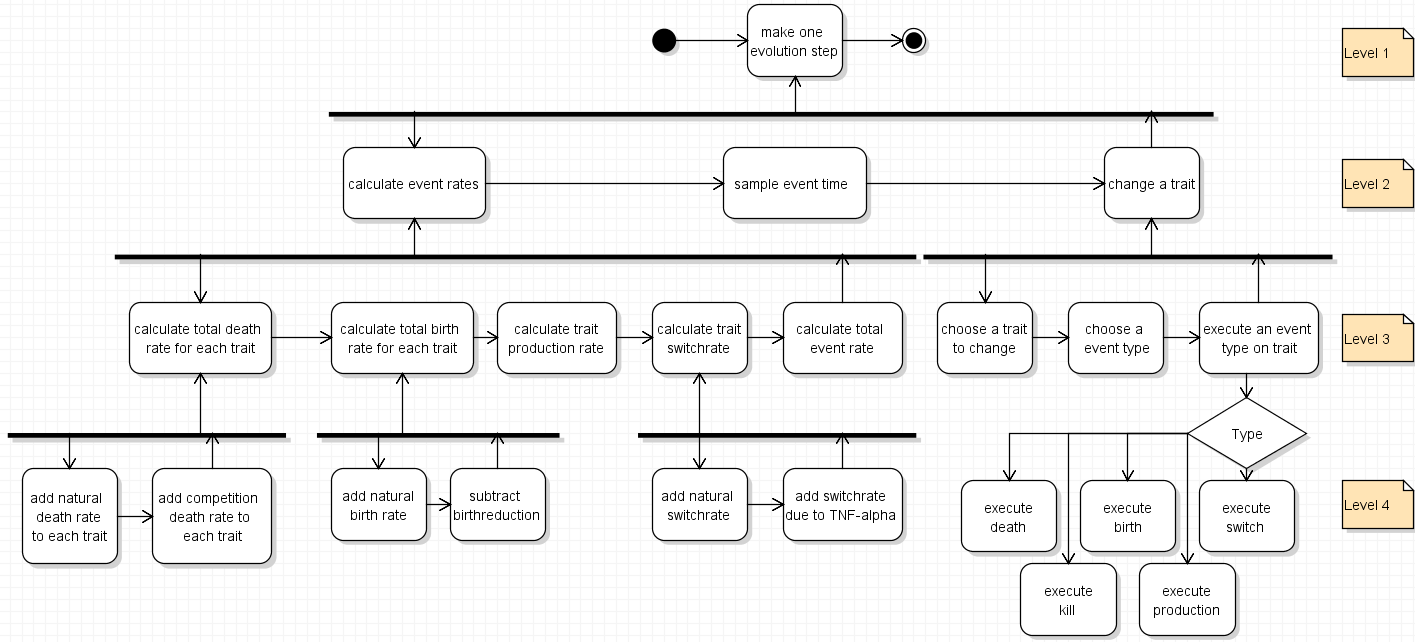
\includegraphics[width=1\linewidth]{../UML/Tiefendiagram}
	\caption{Depth-diagram}
	\label{fig:Tiefendiagram}
\end{figure}

\section{Abstraction level one}
In this and the following chapters I will try to explain the behaviour for each responsibility in the different abstraction levels (see fig. \ref{fig:Tiefendiagram}).
	\subsection{makeEvolutionStep()}
	The top level contains only 'makeEvolutionStep()' with the primary functionalities:
	\begin{enumerate}
		\item '\textbf{calculateTotalEventRates}()': This function calculates all rates (like dying, switch etc.), which together form a total rate for the first event.
		\item '\textbf{samlpleEventTime}()': The 'total event rate' from point 1 is the parameter for a exponentially distributed random variable to sample the time for the next occasion. 
		\item '\textbf{changePopulation}()': Finally the Population will be changed. The function uses the rates that were calculated in the first function to decide who will be affected and what happens to him. \\
	\end{enumerate}
	After this evolutionary step of the population, the point set will be updated with the change made to the population. After the desired steps, point set will be plotted in the graphical user interface.\\
	The algorithmic code should be self-explaining:
	\begin{lstlisting} 
	void PopulationManager::makeEvolutionStep()
	{
	    calculateTotalEventRates();
	    sampleEventTime();
	    changePopulation();
	}
	\end{lstlisting}

\section{Abstraction level two}
	\subsection{calculateTotalEventRates()}\label{subsec:calcRates}
	This function requests the population to calculate all interesting rates. So it calls:
	\begin{enumerate}
		\item '\textbf{calculateTraitDeathRates}()': Provides death rates for each trait. They contain natural and competition deaths.
		\item '\textbf{calculateTraitBirthRates}()': Provides birth rates for each trait. They contain natural birth rates and the reduction.
		\item '\textbf{calculateTraitProductionRates}()': Provides production rates for each t-cell. 
		\item '\textbf{calculateTraitSwitchRates}()': Provides switch rates for each melanoma cell. They contain natural and competition switches.
		\item '\textbf{calculateTraitKillRates}()': Provides kill rates for each t-cell. 
		\item '\textbf{calculateTraitRates}()': Provides overall rates for each trait. This is the rate that something (all rates together) happens to this trait.
		\item And finally the new \textbf{totalEventRate} made from all trait rates. \\
	\end{enumerate}	
	The function was separated to split the responsibilities of the calculation. First it calculates all trait specific rates with 'calculateTotalTraitRates()' and than the total event rate for the first occasion in the for loop. It uses a container named 'traits' that contains all specific traits with their properties. Each trait object in the container specifies his individual population size and rates.
	\begin{lstlisting} 
	void PopulationManager::calculateTotalEventRates()
	{
	    calculateTotalTraitRates();
	    totalEventRate = 0; // resets the last event rate
	    for(TraitClass trait: traits)
	        totalEventRate += trait.TraitRate;
	}
	\end{lstlisting}
	\begin{lstlisting} 
	void PopulationManager::calculateTotalTraitRates()
	{
	    calculateTraitDeathRates();
	    calculateTraitBirthRates();
	    calculateTraitProductionRates();
	    calculateTraitSwitchRates();
	    calculateTraitKillRates();
	    calculateTraitRates();
	}
	\end{lstlisting}	
		
	\subsection{sampleEventTime()} \label{subsec:sample}
	This should be self-explaining. The 'dice' class mas a method called 'rollExpDist($ \lambda $)' that samples $ x \sim exp(\lambda) $. Obviously the eventTime doesn't contain the total time line. It represents the time between the occasions.\\
	I will not describe the functionality of my dice object because its responsibility doesn't belong to the algorithm, but you can be assured that it has been tested very accurately before it was put into use.
	\begin{lstlisting} 
	void PopulationManager::sampleEventTime()
	{
	    event.eventTime = dice.rollExpDist(totalEventRate);
	}
	\end{lstlisting}
	
	\subsection{changePopulation()} \label{subsec:changePop}
	To change the population, we first have to be sure that there is a need for changing. If there is no positive total Event Rate, the population has no reason to look for changes. That's the job of the first if statement. The names of the functions in the statement should clearly state their job description.
	\begin{lstlisting} 
	void PopulationManager::changePopulation()
	{
	    if(totalEventRate > 0){
	        choseTraitToChange();
	        choseEventType();
	        executeEventTypeOnTrait();
	    }
	}
	\end{lstlisting}
	\begin{enumerate}
		\item '\textbf{choseTraitToChange}()': The total event rate is made from all trait rates. This trait rates are used to decide witch trait triggered the event. The decision process is pictured in (fig. \ref{fig:SelectTrait}).
		\item '\textbf{choseEventType}()': To chose the event type that occurs with the chosen trait, we will do the same as before in (fig. \ref{fig:SelectTrait}), but instead of the total event rate we use the total trait rate and the intervals will be the different event rates from that the total trait rate was made (death, birth, siwtch etc.).
		\item '\textbf{executeEventTypeOnTrait}()': This function decides what population changing method should be called based on the event type. More on this in the next level.
	\end{enumerate}
	
	\begin{figure}
		\centering
		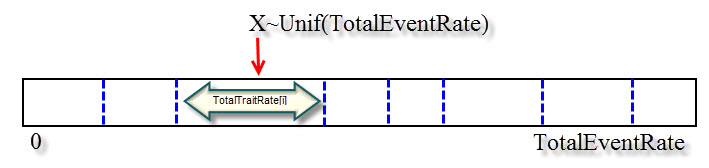
\includegraphics[width=1\linewidth]{Bilder/SelectTrait}
		\caption{uniform trait selection}
		\label{fig:SelectTrait}
	\end{figure}
	
\section{Abstraction level three}
	\subsection{calculating specific rates}
	This subsection summarizes the details of specific rate calculations that were mentioned in (\nameref{subsec:calcRates}).
		\subsubsection{calculateTraitDeathRates()}
		The first for loop resets the last death rate of each trait. Than the natural deaths will be added. They aren't depending on other traits like the competition death rates. The order of these two isn't important.
		\begin{lstlisting} 
		void PopulationManager::calculateTraitDeathRates()
		{
		    for(TraitClass& trait : traits)
		        trait.TraitDeathRate = 0;
		    addNaturalDeathRates();
		    addCompetitionDeathRates();
		}
		\end{lstlisting}
		
		\subsubsection{calculateTraitBirthRates()}
		Like before the last birth rate for each trait has to be reset in the for loop. After this the natural birth rate will be added. Then each member of the population will reduce the this natural birth rate with 'subtractBirthReduction()'.
		\begin{lstlisting} 
		void PopulationManager::calculateTraitBirthRates()
		{
		    for(TraitClass& trait : traits)
		        trait.TraitBirthRate = 0;
		    addNaturalBirthRates();
		    //addMutationalBirthRates();
		    subtractBirthReduction();
		}
		\end{lstlisting}
		There is also a commented line '//addMutationalBirthRates();'. It indicates that it would be possible to change the algorithm with adding the mutational births to the birthrate in this place. A working algorithm for this already exists but would be inefficient (yet neatly arranged).
		
		\subsubsection{calculateTraitProductionRates()}
		To calculate the production of the t-cells, we first have to determine first how each melanoma population effects this production.\\
		To achieve this we first count all effecting melanoma cells for each t-cell type. This is done in the first for-statement (line 4-8). The resulting amount is stored in the 'melCells' vector (initialized in line 3 with size of t-cells and values 0).
		The next for loop (line 9-11) calculates the trait production rate (t-cell production rate) for each trait with the product of the t-cell members, the effecting melanoma cells and the t-celltype specific production rate (line 10).
		\begin{lstlisting} 
		void PopulationManager::calculateTraitProductionRates()
		{
		    vector<double> melCells(tCells,0);
		    for(size_t i = 0; i < tCells; ++i){
		        for(size_t j = 0; j < genotypes * phenotypes; ++j)
		            if(tCellKillRate[i][j] > 0)
		                melCells[i] += traits[1 + tCells + j].Members;
		    }
		    for(size_t i = 1; i <= tCells; ++i){
		        traits[i].TraitProductionRate = traits[i].Members * melCells[i-1] * traits[i].ProductionRate;
		    }
		}
		\end{lstlisting}
		It might be \textbf{confusing to track the indices}. The 'traits' container contains all traits without knowing the difference between them. Thats why we have to know that the first one in the container (traits[0]) is the TNF-$ \alpha $ population, the next are all t-cell populations and then the melanoma cells ( 'traits' contains 1 + t-celltypes + genotypes $ \times $ phenotypes trait objects).
		
		\subsubsection{calculateTraitSwitchRates()}
		The switch rate also consists of natural and competition switch rates. The competition switch rate is effected by the amount of TNF-$ \alpha $.
		\begin{lstlisting} 
		void PopulationManager::calculateTraitSwitchRates()
		{
		    for(TraitClass& trait : traits)
		        trait.TraitSwitchRate = 0;
		    addNaturalSwitchRates();
		    addCompetitionSwitchRates();
		}
		\end{lstlisting}

		\subsubsection{calculateTraitKillRates()}
		These rates belong to the t-cells and describe how fast they are killing the melanoma cells. You can see on the influence for each t-cell type by the melanoma cells in line 6. And in line 8 we see the linear influence of the t-cell type population size on the rate.
		\begin{lstlisting}
		void PopulationManager::calculateTraitKillRates()
		{
		    for(size_t i = 0; i < tCells; ++i){
		        traits[1 + i].TraitKillRate = 0;
		        for(size_t j = 0; j < genotypes * phenotypes; ++j){
		            traits[1 + i].TraitKillRate += tCellKillRate[i][j] * traits[1 + tCells + j].Members;
		        }
		        traits[1 + i].TraitKillRate *= traits[1 + i].Members;
		    }
		}
		\end{lstlisting}

		\subsubsection{calculateTraitRates()}
		Here you can track that the trait rate describes the event triggering rate of a specific trait. The for loop iterates over each trait in 'traits'. The '\&' is important to address the real trait values and not just copies of it.
		\begin{lstlisting} 
		void PopulationManager::calculateTraitRates()
		{
		    for(TraitClass& trait: traits){
		        trait.TraitRate = 0;
		        trait.TraitRate += trait.TraitDeathRate;
		        trait.TraitRate += trait.TraitBirthRate;
		        trait.TraitRate += trait.TraitProductionRate;
		        trait.TraitRate += trait.TraitSwitchRate;
		        trait.TraitRate += trait.TraitKillRate;
		    }
		}
		\end{lstlisting}
		
	\subsection{chose trait, chose event and execute}
	This subsection summarizes how we decide what event trigged the sampled time on which trait at the sampled time. You can find the time sampling in (\nameref{subsec:sample}). The following functions are executed in (\nameref{subsec:changePop}).
		
		\subsubsection{choseTraitToChange} \label{subsubsec:choseTrait}
		The first if statement (line 3) is for testing purpose so that this function can be tested individually. But the total event rate $ > 0 $ was already ensured in (\nameref{subsec:changePop}) so it could be left out without expecting errors.\\
		We use the decision process from the (\nameref{fig:SelectTrait}, fig. \ref{fig:SelectTrait}) to chose the trait that triggered a event. This process begins with sampling $ X \sim Unif[0,r] $, r = totalEventRate in line 4.\\
		The next for loop (line 5-11) represents the decision whether the current trait rate interval was hit by $ X $ or not.
		\begin{lstlisting} 
		void PopulationManager::choseTraitToChange()
		{
		    if(totalEventRate == 0){event.chosenTrait = 0; return;} // update: redundant
		    double HittenTrait = dice.rollContUnifDist(totalEventRate);
		    for(size_t i = 0; i < populations; i++){
		        if(HittenTrait <= traits[i].TraitRate){
		            event.chosenTrait = i;
		            return;
		        }
		        HittenTrait -= traits[i].TraitRate;
		    }
		}
		\end{lstlisting}

		\subsubsection{choseEventType} \label{subsubsec:choseEvent}
		First I would like to say that this function can be done more nicely. To ensure that this functionality is also self-explaining and is 'well written code', it could be implemented as a state pattern to switch the behaviour. Other patterns would also work (strategy/command pattern etc.), but the state pattern would nicely work with the next functionality. \\
		Here you can find a very nice and simple (german) introduction to this pattern (http://www.philipphauer.de/study/se/design-pattern/state.php).\\
		
		This method chooses the event type that was triggered by the chosen trait from before. The idea is the same as before (\nameref{fig:SelectTrait}, fig. \ref{fig:SelectTrait}). This time we use r = TraitRate instead of r = totalEventRate for sampling $ X \sim Unif[0,r] $. This is done in line 4.\\
		Then we again decide which event interval was hit by $ X $. But it's not so easy to access the intervals in a for loop, that's why they where tested individually. The 'if' and 'else if' are passing until the first event decision returns true. The decision process is attached below the code.
		\begin{lstlisting} 
		void PopulationManager::choseEventType()
		{
		    size_t i = event.chosenTrait;
		    double HittenEvent = dice.rollContUnifDist(traits[i].TraitRate);
		
		    if(decideIfEventTimeWasHitten(HittenEvent,traits[i].TraitDeathRate,DEATH)){}
		    else if(decideIfEventTimeWasHitten(HittenEvent,traits[i].TraitBirthRate,BIRTH)){}
		    else if(decideIfEventTimeWasHitten(HittenEvent,traits[i].TraitSwitchRate,SWITCH)){}
		    else if(decideIfEventTimeWasHitten(HittenEvent,traits[i].TraitProductionRate,PRODUCTION)){}
		    else if(decideIfEventTimeWasHitten(HittenEvent,traits[i].TraitKillRate,KILL)){}
		    else if(totalEventRate == 0){event.type = NONE;}
		    else throw (string) "No Event was hit! Trait rate roll was bigger than the trait rate!";
		}
		\end{lstlisting}
		This is the decision process (it is equal to \nameref{subsubsec:choseTrait} line 6-10):
		\begin{lstlisting} 
		bool PopulationManager::decideIfEventTimeWasHitten(double &HittenEvent, double &ChosenEventRate, EventType type)
		{
		    if(HittenEvent < ChosenEventRate){
		        event.type = type;
		        return true;
		    }
		    HittenEvent -= ChosenEventRate;
		    return false;
		}
		\end{lstlisting}
		
		\subsubsection{executeEventTypeOnTrait} \label{subsubsec:executeEvOnTr}
		Here we decide on the basis of the event type what we will do to the population. This decision is visualized in the (\nameref{fig:Tiefendiagram}) by the diamond with the decision parameter 'Type' which in our case is the 'event.type'.
		\begin{lstlisting}
		void PopulationManager::executeEventTypeOnTrait()
		{
		    if(event.type == DEATH){traits[event.chosenTrait].Members -= 1.;}
		    else if(event.type == BIRTH){executeBirth();}  
		    else if(event.type == SWITCH){executeSwitch();} 
		    else if(event.type == PRODUCTION){executeProduction();} 
		    else if(event.type == KILL){executeKill();}   
		    else if(event.type == NONE){}
		    else throw (string) "No event type has been chosen before: executeEventTypeOnTrait()";
		}
		\end{lstlisting}
		The 'throw' statement in the else part is already unnecessary. It simply throws a custom exception if the event type has no valid value. But this can't happen, so it can be left out. In fact it should be deleted because it counts as a very light version of dead code which is known as a 'code smell'.\\
		This many 'if' and 'else if' statements are not very nice and can easily be replaced by a (switch, case) statement. This would look like this:
		\begin{lstlisting}
		void PopulationManager::executeEventTypeOnTrait()
		{
			switch (event.type){
			case BIRTH:
				executeBirth();
				break;
			case SWITCH:
				executeSwitch();
				break;				
			case PRO...
				...
			}
		}
		\end{lstlisting}
		
\section{Abstraction level four}
This section describes the details of some functions of level three with more than one responsibility.
	\subsection{death rate details}
	The death rate is composed of the natural deaths and the competition deaths.
		\subsubsection{addNaturalDeathRates()}
		Each member of a trait has a constant natural death rate. Line 4 should be self-explaining.
		\begin{lstlisting}
		void PopulationManager::addNaturalDeathRates()
		{
		    for(TraitClass& trait : traits)
		        trait.TraitDeathRate += trait.Members * trait.DeathRate;
		}
		\end{lstlisting}
		
		\subsubsection{addCompetitionDeathRates()}
		To observe the competition deaths, we iterate over each member of the population (for-loop in line 4) and consider the competition effect (for-loop in line 6) for each member of the population (line 9).
		\begin{lstlisting}
		void PopulationManager::addCompetitionDeathRates()
		{
		    double sum;
		    for(size_t i = 0; i < populations; ++i){
		        sum = 0;
		        for(size_t j = 0; j < populations; ++j){
		            sum += competition[i][j] * traits[j].Members;
		        }
		        traits[i].TraitDeathRate += sum * traits[i].Members;
		    }
		}
		\end{lstlisting}		
		
	\subsection{birth rate details}
	The birth rate is composed of the natural births and the birth reduction.
		\subsubsection{addNaturalBirthRates()}
		Natural births are very straight forward like the natural deaths.
		\begin{lstlisting}
		void PopulationManager::addNaturalBirthRates()
		{
		    for(TraitClass& trait : traits)
		        trait.TraitBirthRate += trait.Members * trait.BirthRate;
		}
		\end{lstlisting}
		
		\subsubsection{subtractBirthReduction()}
		There is also an birth reducing effect for each new member of a trait. This reducing effect gets calculated in the for loop line 6-8 and effects the birth rate for this trait in line 9.\\
		This may cause the birth rate for the trait to be negative what would lead to problems to technically process the concept of (fig. \ref{fig:SelectTrait}) which is used in (\nameref{subsubsec:choseTrait} and \nameref{subsubsec:choseEvent}). This justifies the need of line 11-12.
		\begin{lstlisting}
		void PopulationManager::subtractBirthReduction()
		{
		    double sum;
		    for(size_t i = 0; i < populations; ++i){
		        sum = 0;
		        for(size_t j = 0; j < populations; ++j){
		            sum += birthReduction[i][j] * traits[j].Members;
		        }
		        traits[i].TraitBirthRate -= sum * traits[i].Members;
		        
		        if(traits[i].TraitBirthRate < 0)
		            traits[i].TraitBirthRate = 0;
		    }
		}
		\end{lstlisting}		
		
	\subsection{switch rate details}
	The switch rate is composed of the natural switch and the switch due to TNF-alpha. 
		\subsubsection{addNaturalSwitchRates()}
		The switch rate matrix differs for each genotype. That's why we need three for loops (2 loop $ \to $ matrix, 3 loops $ \to $ tensor 3rd dim). Within the first for loop we see the usual behaviour to calculate the switch rate for the k.th genotype. It calculates the effect switch rate to make a switch for each member (line 6-7) and considers that for the entire trait in line 9-10. The '+=' in line 10 can also be a '='. But the '+=' symbolizes that there is also a competition rate as a part of the trait switch rate. In this version both (addNaturalSwitchRates and addCompetitionSwitchRates) don't need to be executed in a particular order ($ \to $ more independency).
		\begin{lstlisting}
		void PopulationManager::addNaturalSwitchRates()
		{
		    double switchrate;
		    for(size_t k = 0; k < genotypes; ++k){
		        for(size_t i = 0; i < phenotypes; ++i){
		            switchrate = 0;
		            for(size_t j = 0; j < phenotypes; ++j) // Improve: reuse!
		                switchrate += naturalSwitch[k][i][j];
		            switchrate *= traits[getMelanomIndex(k,i)].Members;
		            traits[getMelanomIndex(k,i)].TraitSwitchRate += switchrate;
		        }
		    }
		}
		\end{lstlisting}	
		There is one comment 'Improve:...'. It states a simple improvement that can be made by calculating the inner for loop (line 7-8) once the simulation starts, because its the same calculation each step. If you would like to have this improvement than please contact me and I send you the updated version.
			
		\subsubsection{addCompetitionSwitchRates()}\label{subsubsec:addCompSwitch}
		First I would like to emphasise that in the old version, the 'traitNumber' variable in this function is a relict before there was a 'getMelanomIndex(k,i)' method. If you got the version with the 'traitNumber' than please simply delete it because I has no effect on the algorithm. As you can see below it get only incremented but never used. The less confusing algorithm is the second code snippet.\\
		In general there is one issue with this calculation. It is very similar to the natural rate with additional influence of TNF-$ \alpha $ in line 9 (and competition instead of natural rate). That's why there is a simple way to increase the efficiency by adding the additional increment after the natural switchrate. You can find this approach in the third code snippet.\\
		I assume that this happened because I stopped working after the natural switch rates were tested and implemented and started the competition switch rates the next morning.\\
		Snippet with dead code:
		\begin{lstlisting}
		void PopulationManager::addCompetitionSwitchRates()
		{
		    size_t traitNumber;
		    double switchrate;
		    for(size_t k = 0; k < genotypes; ++k){
		        traitNumber = k * phenotypes;
		        for(size_t i = 0; i < phenotypes; ++i){
		            traitNumber += i;
		            switchrate = 0;
		            for(size_t j = 0; j < phenotypes; ++j)
		                switchrate += competitionSwitch[k][i][j];
		            switchrate *= traits[getMelanomIndex(k,i)].Members * traits[0].Members;
		            traits[getMelanomIndex(k,i)].TraitSwitchRate += switchrate;
		        }
		    }
		}
		\end{lstlisting}
		Snippet without dead code:
		\begin{lstlisting}
		void PopulationManager::addCompetitionSwitchRates()
		{
		    double switchrate;
		    for(size_t k = 0; k < genotypes; ++k){
		        for(size_t i = 0; i < phenotypes; ++i){
		            switchrate = 0;
		            for(size_t j = 0; j < phenotypes; ++j)
		                switchrate += competitionSwitch[k][i][j];
		            switchrate *= traits[getMelanomIndex(k,i)].Members * traits[0].Members;
		            traits[getMelanomIndex(k,i)].TraitSwitchRate += switchrate;
		        }
		    }
		}
		\end{lstlisting}
		The improved code would be:
		\begin{lstlisting}
		void PopulationManager::addSwitchRatesImproved()
		{
		    double natSwitchSum;
		    double compSwitchSum;
		    for(size_t k = 0; k < genotypes; ++k){
		        for(size_t i = 0; i < phenotypes; ++i){
		            natSwitchSum = 0;
		            compSwitchSum = 0;
		            for(size_t j = 0; j < phenotypes; ++j){
		                natSwitchSum += naturalSwitch[k][i][j];;
		                compSwitchSum += competitionSwitch[k][i][j];
		            }
		            natSwitchSum *= traits[getMelanomIndex(k,i)].Members;
		            compSwitchSum *= traits[getMelanomIndex(k,i)].Members * traits[0].Members;
		            traits[getMelanomIndex(k,i)].TraitSwitchRate = natSwitchSum + compSwitchSum;
		        }
		    }
		}
		\end{lstlisting}
		Attention: I haven't tested the improved code. If you want to have this improvement (it could increase the efficiency noticeably), please contact me about this matter. I simply don't want to force a newer version of the simulator if the current version already works fine and is already modified by you.
	
	\subsection{execute event type details}
	Here we see how the events getting executed on the chosen traits (except the killing event. This trait rather executes than getting executed $\ddot\smile$). (see \nameref{subsubsec:executeEvOnTr})
		\subsubsection*{execute death}
		This is simply one line and doesn't deserve is own function. That's why it gets executed directly in (\nameref{subsubsec:executeEvOnTr}).
		\begin{lstlisting}
			traits[event.chosenTrait].Members -= 1.;
		\end{lstlisting}

		\subsubsection{executeBirth()}
		Here comes the influence of a mutation. While a birth can be triggered from the chosen trait, it still can be a mutant and belong to another genotype. 
		%In case the trait that is giving birth is a t-cell, than automatically a TNF-alpha gets produced. That's why we execute the production in line 4. 		
		If its a melanoma cell (or a TNF-$ \alpha $) than we can simply ask 'isMutation()' if its a mutant or not(TNF-$ \alpha $'s and t-cells mutation probability gets initialized with zero). In case of mutation the function 'choseMutantGenotype' redirects the chosenTrait to the mutant trait. I will attach both ('isMutation()' and 'choseMutantGenotype') snippets after the birth method.
		\begin{lstlisting}
		void PopulationManager::executeBirth()
		{
			if(isMutation()){
		        choseMutantGenotype();
		        traits[event.chosenTrait].Members++;
		    }
			else{
		        traits[event.chosenTrait].Members++;
		    }
		}
		\end{lstlisting}
		Below you see the decision if its a mutation or not. It simply considers the mutation probability of the chosen trait (only the melanoma cells have positive probabilities $ \to $ in fact only the genotypes have differ from each other). The comment shows that this decision can be done in one line but would not be so overseeable.
		\begin{lstlisting}
		bool PopulationManager::isMutation()
		{
		    double roll = dice.rollContUnifDist(1);
		    if(roll < traits[event.chosenTrait].Mutation)
		        return true;
		    else
		        return false;
			//return roll < traits[event.chosenTrait].Mutation ? true : false;		        
		}
		\end{lstlisting}
		To chose the mutant after we know that there will be a mutant is again done with (\nameref{fig:SelectTrait}, fig. \ref{fig:SelectTrait}).\\
		First we select the genotype and phenotype of the chosen trait in line 3 and 4 (you can look the functions up in the source code). Than we sample $ X \sim Unif([0,1]) $ (line 6) and chose the intervals like the ones in the given mutation kernel (line 9). This procedure should familiar by now.
		\begin{lstlisting}
		void PopulationManager::choseMutantGenotype()
		{
		    size_t chosenGenotype = getGenotypeOfTraitIndex(event.chosenTrait);
		    size_t chosenPhenotype = getPhenotypeOfTraitIndex(event.chosenTrait);
		    size_t mutantGenotype = 0;
		    double HittenTrait = dice.rollContUnifDist(1);
		
		    for(mutantGenotype = 0; mutantGenotype < genotypes; ++mutantGenotype){
		        if(HittenTrait <= mutationKernel[chosenGenotype][mutantGenotype])
		            break;
		        HittenTrait -= mutationKernel[chosenGenotype][mutantGenotype];
		    }
		    event.chosenTrait = getMelanomIndex(mutantGenotype, chosenPhenotype); 
		}
		\end{lstlisting}
		
		\subsubsection{executeSwitch()}
		This function is rather simple, but the 'getSwitchedTrait()' call gets a bit confusing because there are many linebreaks. If you look it up in the code editor than it will be much more readable.\\
		\begin{lstlisting}
		void PopulationManager::executeSwitch()
		{
		    size_t switchedTrait = getSwitchedTrait();
		    traits[event.chosenTrait].Members--;
		    traits[switchedTrait].Members++;
		}
		\end{lstlisting}
		Below you see 'getSwitchedTrait()' which finds the switched trait among the genotype (the chosen trait will switch to the switched trait). It is very recommended to look at this method in the Qt Creator or another editor.\\
		In line 3 we sample $ X \sim Unif([0,r]) $ with $ r = \frac{TraitSwitchRate[k]}{Members[k]} $. Where $ k $ represents the chosen trait index. This gives us the actual switchrate for one member (consisting of the natural rates and the competition rates times the TNF$ -\alpha $).\\
		Than we determine the genotype and phenotype of the chosen trait in line 4 and 5. In the for loop we consider each possible phenotype to switch to. In line 7 you can see that the switchrate for the considered switchable trait gets calculated and like before in \nameref{fig:SelectTrait} (fig. \ref{fig:SelectTrait}), we decide of this switchrate caused the switch. It this was the case than we return the current considered phenotype as switch destination.
		\begin{lstlisting}
		size_t PopulationManager::getSwitchedTrait()
		{
		    double HittenSwitch = dice.rollContUnifDist(traits[event.chosenTrait].TraitSwitchRate/traits[event.chosenTrait].Members);
		    size_t chosenGenotype = getGenotypeOfTraitIndex(event.chosenTrait);
		    size_t chosenPhenotype = getPhenotypeOfTraitIndex(event.chosenTrait);
		    for(size_t switchPhenotype = 0; switchPhenotype < phenotypes; ++switchPhenotype){
		        double currentSwitchRate = getSpecificSwitchRate(chosenPhenotype, chosenGenotype, switchPhenotype);
		        if(HittenSwitch <= currentSwitchRate)
		            return getMelanomIndex(chosenGenotype, switchPhenotype);
		        HittenSwitch -= currentSwitchRate;
		    }
		    throw (string) "getSwitchedTrait() could not find a matching switch!";
		    return 0;
		}
		\end{lstlisting}
		
		\subsubsection{executeProduction()}
		If a t-cells gets produced, than there appear 'ProductionAmount' (depending on the chosen t-cell) new TNF-$ \alpha $'s and the t-cell population increases by one.
		\begin{lstlisting}
		void PopulationManager::executeProduction()
		{
		    traits[0].Members += traits[event.chosenTrait].ProductionAmount;
		    traits[event.chosenTrait].Members++;
		}
		\end{lstlisting}
		
		\subsubsection{executeKill() - unfinished}
		Self-explaining.
		\begin{lstlisting}
		void PopulationManager::executeKill()
		{
		    traits[getKilledTrait()].Members--;
		    traits[0].Members += TNFsAfterKill;
		}
		\end{lstlisting}
		This is again better in the editor, else the linebreaks may cause confusion.
		\begin{lstlisting}
		size_t PopulationManager::getKilledTrait()
		{
		    double HittenCell = dice.rollContUnifDist(traits[event.chosenTrait].TraitKillRate/traits[event.chosenTrait].Members);
		    size_t tcell = event.chosenTrait -1;
		    for(size_t i = 0; i < genotypes*phenotypes; ++i){
		        if(HittenCell < tCellKillRate[tcell][i] * traits[1+ tCells + i].Members)
		            return 1+tCells+i;
		        HittenCell -= tCellKillRate[tcell][i] * traits[1+ tCells + i].Members;
		    }
		    throw (string) "no killed trait found!";
		    return 0;
		}
		\end{lstlisting}								

\section{Background Information}
	\subsection{Parameter Input} \label{subsec:PaInput}
	This section reminds (very brief) how the input of the simulator has to be and how it gets processed.\\
	There exists a 'MusterInstanz' and a 'Testinstanz\_kommentiert' file in the repository and in the milestone 1.1.4. The first explains the structure of the parameter files and the second gives an example of this. You can observe the second file in (fig. \ref{fig:CommentedParameterfile}). Make sure you know how to read the 'Deathratematrix due T-cell resistance'.
	\begin{figure}
		\centering
		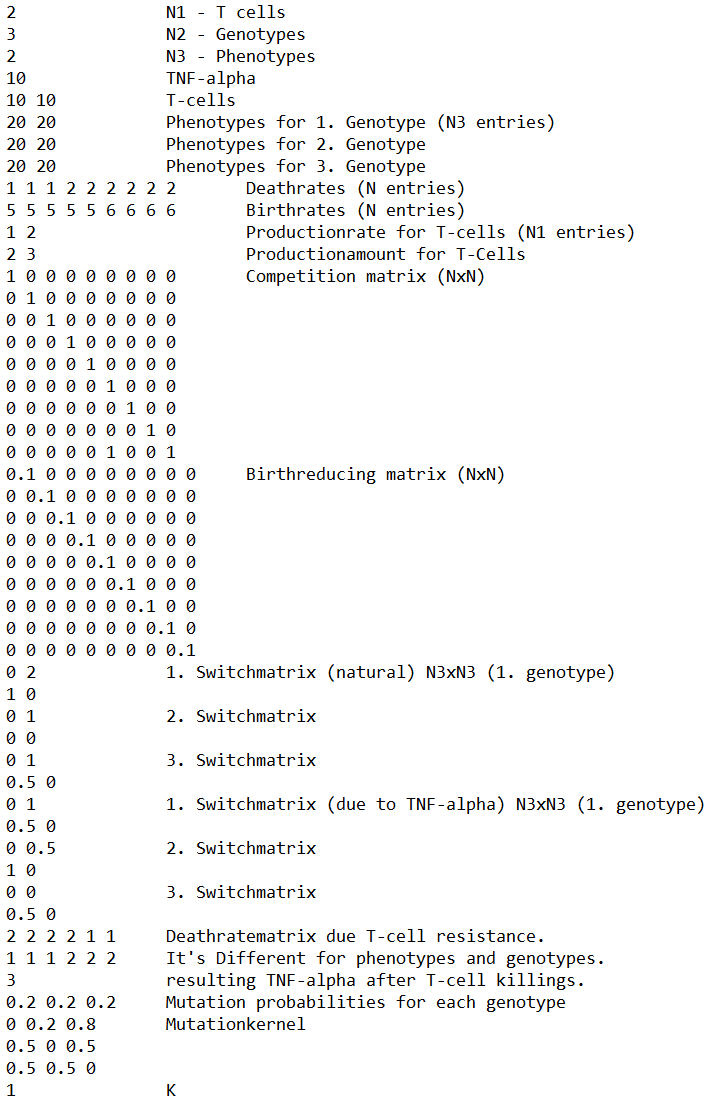
\includegraphics[width=0.9\linewidth]{Bilder/CommentedParameterfile}
		\caption{Testinstanz\_kommentiert}
		\label{fig:CommentedParameterfile}
	\end{figure}
	The Parameters were read with my own builded 'CFileStreamer' that can be seen in the source files. But in general its not important. In the following snippet you see how the Parameters are processed. In line 3-4 the streaming object of the desired file gets created. It contains all informations as a string. In each function line 5-12 it iterates over the strings in the stream and stores the expected parameters.
	\begin{lstlisting}
	void PopulationManager::initWithFile(const string FName)
	{
	    CFileStreamer object(FName);
	    IFileStreamer& stream(object);
	    readPopulations(stream);
	    createTraits(stream);
	    readDeathBirthProductionRates(stream);
	    readCompetition(stream);
	    readBirthReduction(stream);
	    readNaturalCompetitionSwitchRates(stream);
	    readTCellKillRateAndAmount(stream);
	    readMutationWithKernel(stream);
	    K = std::stod(stream.getNextWord()); // Read K from filestream
	    applyKToParameters();
	}
	\end{lstlisting}

	\subsection{Influence of K}
	As you maybe noticed, there is nothing about the influence of the K. The simulation itself doesn't use the K to iterate the algorithm. The K gets applied when the parameters were read and after the algorithm has finished its work. In '\nameref{subsec:PaInput}' you can see in the code snipped line 14 that the K gets applied to the parameters after they are known. In the following snipped you can observe what happens.
	\begin{lstlisting}
	void PopulationManager::applyKToParameters()
	{
	    for(TraitClass& trait : traits){ // Members and ProductionRates
	        trait.Members *= K;
	        trait.ProductionRate /= K;
	    }
	    for(size_t i = 0; i < populations; ++i){    // competition death
	        for(size_t j = 0; j < populations; ++j)
	            competition[i][j] /= K;
	    }
	    for(size_t i = 0; i < populations; ++i){    // birth reduction
	        for(size_t j = 0; j < populations; ++j)
	            birthReduction[i][j] /= K;
	    }
	    for(size_t k = 0; k < genotypes; ++k){      // competition switch
	        for(size_t i = 0; i < phenotypes; ++i){
	            for(size_t j = 0; j < phenotypes; ++j)
	                competitionSwitch[k][i][j] /= K;
	        }
	    }
	    for(size_t i = 0; i < tCells; ++i){         // killRate
	        for(size_t j = 0; j < phenotypes * genotypes; ++j)
	            tCellKillRate[i][j] /= K;
	    }
	}
	\end{lstlisting}	
	To ensure that the plot shows the population with the desired K, it accesses the members of the trait only through a special accessor method:
	\begin{lstlisting}
	double PopulationManager::getKMembers(int TraitIndex) const
	{
	    return traits[TraitIndex].Members / K;
	}
	\end{lstlisting}
	Unfortunately it would be far to expensive to document the actual plotting process and the graphical implementation because it's very technical and even more work than the algorithm itself. Also its much harder to test.
	
	\subsection{Precision problems}
	The precision was chosen to be the standard double precision. Now the interesting question would be, what can cause precision related false data? To answer that I would like to explain what double precision is and what a 'Mantissa' is. \\
	The mantissa is part of a number in scientific notation or a floating-point number, consisting of its significant digits. I.e. of $ 210.45 $ would have the scientific notation $ 2.1045 \times 10^{2}$ where $ 2.1045 $ are the significant digits thus the mantissa. Its also called the significand. \\
	In nearly any case, precision problems are caused by mantissas that get to long. Now, how does a double variable look and when do precision errors occur?
	\begin{figure}
		\centering
		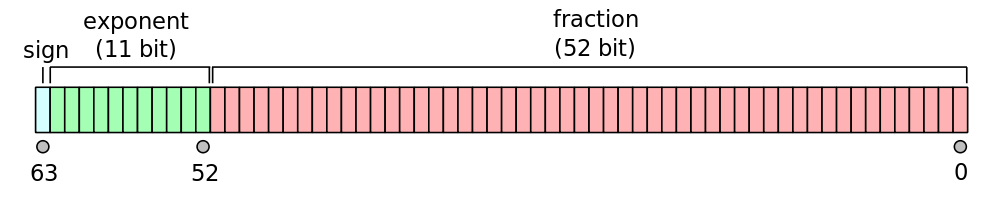
\includegraphics[width=1\linewidth]{Bilder/Double_Floating_Point_Format.png}
		\caption{double precision format \textregistered Codekaizen/Wikimedia}
		\label{fig:Double_Floating_Point_Format}
	\end{figure}
	As you can see in (fig. \ref{fig:Double_Floating_Point_Format}) a double variable can store 63 bits. In our case are only 62 interesting because we don't get negative numbers. The first 11 bits (ignoring the sign) are used to represent the exponent of the scientific notation. In the example of the mantissa this would be $ 2 $ (from $ 2.1045 \times 10^{2}$). This means that the exponent can maximal 2048. In the case of the simulation this is very unlikely to reach. The more interesting matter are the next 52 bits for the mantissa. 52 bits mean that the maximal mantissa can be $ 4503599627370496 $. This means that we can expect the digits to be precise for a mantissa with maximal length $ \log_{10}(2^{53}) = 53\log_{10}(2) \approx 15.95 \approx 16 $.\\
	In short, if the mantissa exceeds 16 digits, than the less important digits will get lost (lowest digits). Normally the exponent doesn't exceed, thus we don't have to worry that the numbers are getting very small or big.

\end{document}
